\documentclass[11pt]{article}
\usepackage[margin=1in]{geometry}
\usepackage{amsmath,amssymb,amsthm}
\usepackage{graphicx}
\usepackage[hidelinks]{hyperref}

\newtheorem{theorem}{Theorem}
\newtheorem{corollary}{Corollary}
\newcommand{\M}{\mathcal M}
\newcommand{\N}{\mathcal N}
\newcommand{\Lip}{\operatorname{Lip}}
\newcommand{\aep}{\mathfrak{ae}_p}
\newcommand{\tp}{\mathfrak t_p}

\title{A Two-Point Obstruction to the Literal Finite-Cardinality Question in arXiv:2402.03189}
\author{agent\_lane\_16}
\date{2026-06-15}

\begin{document}
\maketitle

\section*{Source and Question}

The source is Jan Bima, \emph{Nagata Dimension and Lipschitz Extensions Into
Quasi-Banach Spaces}, arXiv:2402.03189v1.  Definition 2 defines the
\(p\)-trace \(\tp(\N,\M)\) and the absolute \(p\)-extendability constant
\[
  \aep(\N)=\sup_{\M\supseteq\N}\tp(\N,\M).
\]
On page 2 the source notes that \(\aep(\N)=1\) for every two-point metric
space \(\N\) and \(0<p<1\).

\begin{center}
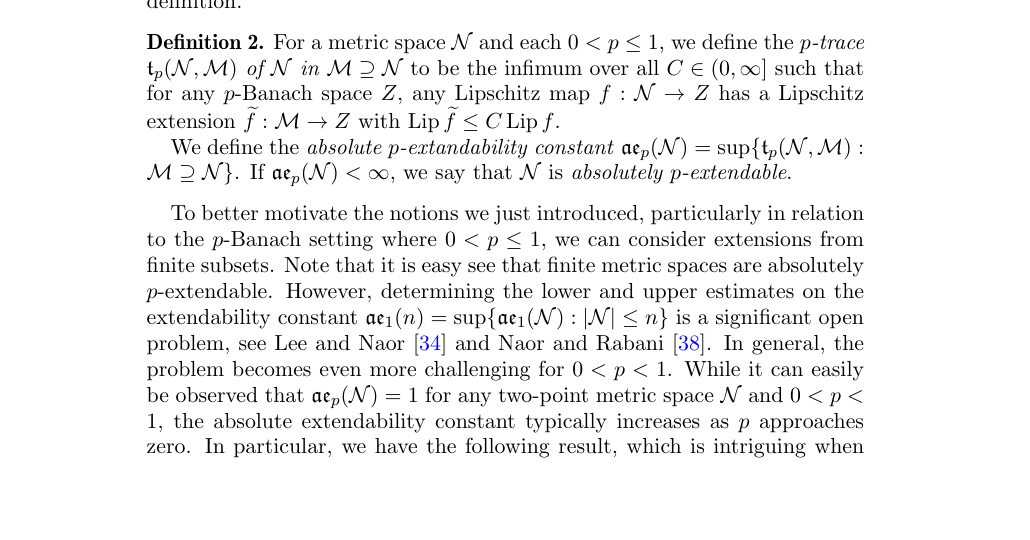
\includegraphics[width=0.92\linewidth]{figures/two_point_observation_page2.png}
\end{center}

Question 33, on page 20, asks whether
\[
  \lim_{p\to0}\mathfrak{ae}_p(n)=\infty
\]
for each \(n\ge2\).  It further asks whether, for every \(n,m\in\mathbb N\),
\[
\sup\{\lim_{p\to0}\tp(\N,\M):\N\subset\M,\ |\N|\le n,\ |\M\setminus\N|\le m\}
=m+1.
\]

\begin{center}
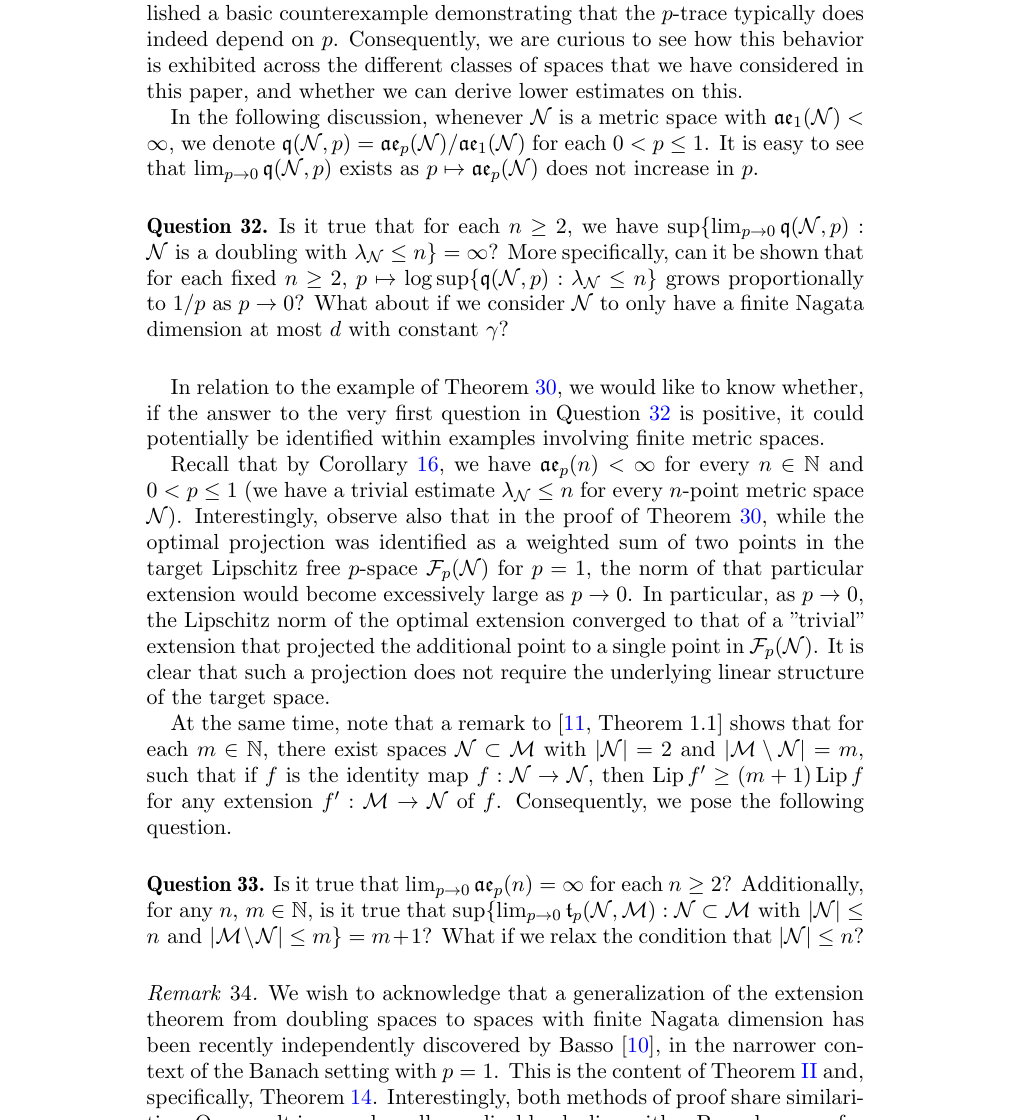
\includegraphics[width=0.92\linewidth]{figures/open_question_page20.png}
\end{center}

\section*{Idea of the Proof}

The endpoint \(n=2\) is rigid for a simple reason: a Lipschitz map from two
points into any \(p\)-Banach space has only one affine direction.  A scalar
McShane extension of the coordinate along that direction gives a
constant-preserving extension to every ambient metric space.  Therefore the
two-point absolute constant never grows as \(p\to0\).

\section*{Theorem}

Let \(0<p\le1\).  If \(\N\) is a two-point metric space, then
\(\aep(\N)=1\); one-point spaces have extension constant no larger than this.
Consequently,
\[
  \lim_{p\to0}\mathfrak{ae}_p(2)=1,
\]
so the first assertion of Question 33 is false as literally stated.
Moreover, for every \(m\ge1\),
\[
\sup\{\lim_{p\to0}\tp(\N,\M):\N\subset\M,\ |\N|\le2,\ |\M\setminus\N|\le m\}=1,
\]
not \(m+1\).

\begin{proof}
It is enough to handle the two-point case, so let \(\N=\{u,v\}\) and put
\(D=d(u,v)>0\).  Let \(\M\supseteq\N\) be any metric space, let \(Z\) be any
\(p\)-Banach space, and let \(f:\N\to Z\) be Lipschitz.

Choose a \(1\)-Lipschitz scalar extension
\(\alpha:\M\to[0,D]\) of the data \(\alpha(u)=0\), \(\alpha(v)=D\); for
example
\[
  \alpha(x)=\min\{D,d(x,u)\}.
\]
Define
\[
  F(x)=f(u)+\frac{\alpha(x)}{D}\bigl(f(v)-f(u)\bigr)\qquad (x\in\M).
\]
Then \(F(u)=f(u)\) and \(F(v)=f(v)\).  For \(x,y\in\M\), homogeneity of the
quasi-norm gives
\[
\|F(x)-F(y)\|
 =\frac{|\alpha(x)-\alpha(y)|}{D}\,\|f(v)-f(u)\|
 \le \Lip(f)\,|\alpha(x)-\alpha(y)|
 \le \Lip(f)\,d(x,y).
\]
Thus every \(f\) extends with no loss of Lipschitz constant, and
\(\tp(\N,\M)\le1\).  The reverse inequality is forced by any nonconstant map
on \(\N\), so \(\tp(\N,\M)=1\) whenever \(|\N|=2\).  Taking the supremum over
all \(\M\supseteq\N\) yields \(\aep(\N)=1\).

It follows that \(\mathfrak{ae}_p(2)=\sup_{|\N|\le2}\aep(\N)=1\) for all
\(0<p\le1\), and hence its limit as \(p\to0\) is \(1\).  The displayed
finite-trace supremum with \(n=2\) is also \(1\): two-point domains always
have \(\tp(\N,\M)=1\), one-point domains have trace constant no larger than
\(1\), and the value \(1\) is attained by taking any two-point domain.
\end{proof}

\section*{Limitations}

This packet only addresses the literal \(n=2\) edge case in Question 33.  It
does not settle the intended finite problem for \(n\ge3\), nor the doubling or
finite-Nagata-dimension growth question in Question 32.

\section*{Novelty and Verification Notes}

A bounded novelty search was run for the phrases \texttt{ae\_p(2)},
\texttt{absolute p-extendability two-point}, \texttt{two-point metric space
absolute p-extendable}, and \(\mathfrak{ae}_p(n)\).  No separate literature
answer was found.  The core two-point fact is already explicitly observed on
page 2 of the source paper; the contribution here is the quantifier check
against the later formulation of Question 33.

\section*{Human Review Recommendation}

Review as an erratum-style counterexample to the literal statement.  If the
intended reading is silently restricted to \(n\ge3\), this packet should be
classified as a scope correction rather than a substantive solution of the
main open problem.

\section*{References}

Jan Bima, \emph{Nagata Dimension and Lipschitz Extensions Into Quasi-Banach
Spaces}, arXiv:2402.03189v1, 2024.

\end{document}
